\captionsetup{font=footnotesize}

\section{Assignment 1} \label{s:intro}

\subsection{Introduction}
    For the first assignment the task is to develop an L1-D-Cache using SystemC. We have been provided with the CPU module, the Memory module, and all the necessary channels employed for communication between the two. For the sake of simplicity, as hinted in the description of the first assignment, I decide not to implement a new Cache module in between the existing Memory and CPU module. Instead, I modified the Memory module to let it simulate the communication with memory and behave as a Cache. As defined in the assignment requirements, the base cache memory size is 32kB (32768 bytes). These are addressed in our simulation model with words of 4 bytes. The cache line size is 32 Bytes, meaning that it will contain 8 words. Furthermore, it is an 8-way-associative cache, meaning that all the available lines are subdivided in sets of 8. The total amount of lines for this cache size is 1024, leading to 128 total sets. 

\subsection{Parameters}
The cache in the model is structured by using C structs as it seems to be the most intuitive way to model the data structure. My model comes with a struct for the CacheLine and for the CacheSet. My cache is defined as a CacheSet cache[NUM\_SETS].
The CacheLine contains a tag, data[8], and two booleans, state and dirty. The first two are straight forward, tag and the data contents (32 bytes), the state indicates whether the line has been used (i.e. allocated and not empty) and not just containing zero, and dirty bit indicates whether the data in the cache was modified and is waiting for a write-back. The CacheSet contains CacheLine lines[8] and agingBits[8], where the 8 lines of the 8-way-associative cache are represented, and the aging bits (one for each line) are there to keep track of which lines to evict with the LRY policy that we are going to mention in the next section. Technically, for a 32kB cache memory, in order to be able to parse the requesting address coming from the CPU, we need the 5 least significant bits for the line offset (where the data in the 32 bytes line is located), following 7 bits for the set, and the rest for the tag. These can be dynamically calculated during runtime for testing with different memory sizes (i.e. if cache line size was to go up to 64bytes, we would require one extra byte for the line offset, and shift all the rest by one).

\subsection{Policies}
    In order to make the cache functioning properly, we need to define some behaviour on how the cache will behave with new entries. Also, when the sets are full, and new data needs to be allocated, we need to decide which lines to evict. As of the description of the assignment, the implemented cache comes with a write-back strategy mixed with write-on-allocate strategy. Additionally, the eviction policy is LRU, or Least Recently Used. 

\subsection{Write-back}
This policy made the work easier as the write-back policy consists in writing modified cache elements to main memory (or higher level caches) not immediately but eventually, any time prior to eviction. In real systems this seems to be done as an asynchronous task, but I model it in a way that the cache line is synced with the memory when it is about to be evicted and it is dirty. In our case this doesn’t have much impact as we are not actually storing any data, nor we are checking the data in the cache lines. In a real case scenario, this would mean, for example, that when we there’s a read miss on a cache line, we would first perform a write of that specific data (not the whole line) to memory to avoid inconsistencies.
\subsection{Write-on-allocate}
    In combination to the write-back policy we implement the write-on-allocate policy, the combination that seems very common in the industry as well. This strategy consists in allocating an entire cache line when a read miss or a write miss occur. Thus, this means that when the eviction happens (or when a read or write miss occurs because of invalid line), the cache will pull an entire block of memory from memory, and if a write is required then it will write on the modified data, setting the dirty bit. 
\subsection{LRU}
The eviction policy adopted is LRU, and is implemented by using the aging bits in the cache lines. In this specific model implementation, the decision was to keep the unused bits as 0s, while all the valid bits would range between 1 and 8, where 8 is the most recent used bit. When a valid line in a full cache set needs to be evicted, the findOldest method will get the index of the line containing aging bit 1, the oldest. After this, if the dirty bit is set, the cache will need to write-back and pull the new cache line and set the dirty bit to zero. The aging bit of the new cache line will be set to max, 8, and all the other aging bits will be decreased by 1. 

\subsection{Results}
    To analyze the performance of our cache model we tested it on provided traces of max\_mul on grid 50x50, 200x200, 5000x8, 8x5000, and fft. Furthermore, these were tested on 3 different memory sizes. As it can be seen in the table below, the changes are in hit rates are not big, but there are some. For instance, with higher cache memory size, smaller workloads seem to benefit as the higher number of sets probably leads to less evictions. However, for in some cases with larger workloads, the performance seems to be a bit unpredictable and even deteriorated with higher memory size. Also, its interesting to observe that 5000x8 and 8x5000 on a 512kB cache have such different results, meaning that the memory access pattern actually influences the performance of the cache, and for 128kB the performance even drops to 88.8% for the 8x5000, which might indicate that its a bad combination in terms of sets number (which is pretty much the only parameter changing).

\usepackage{geometry}
\usepackage{booktabs}

\begin{table}[htbp]
  \centering
  \caption{Performance Measurements}
  \begin{tabular}{cccc}
    \toprule
    \textbf{Size} & \textbf{Configuration} & \textbf{Accuracy (\%)} \\
    \midrule
    32KB & 50x50 & 96.417364 \\
         & 200x200 & 97.764266 \\
         & 5000x8 & 97.815325 \\
         & 8x5000 & 96.767443 \\
         & FFT & 97.913266 \\
    \midrule
    128KB & 50x50 & 99.596832 \\
          & 200x200 & 93.855263 \\
          & 5000x8 & 94.055455 \\
          & 8x5000 & 88.856099 \\
          & FFT & 96.333944 \\
    \midrule
    512KB & 50x50 & 99.865399 \\
          & 200x200 & 98.536427 \\
          & 5000x8 & 98.486753 \\
          & 8x5000 & 97.727058 \\
          & FFT & 99.603731 \\
    \bottomrule
  \end{tabular}
\end{table}

\newpage
\section{Assignment 2}

\subsection{Introduction}
In the previous assignment, a basic bus-based cache coherence system was implemented using SystemC transaction-level modeling (TLM). For the current assignment, the model has been further developed by introducing a bus implementation and making more extensive use of templates. The key change is that most of the channel/port communication has been abstracted away, and the modules now directly access each other's methods (with some exceptions where port communication is still used, such as between the bus and memory).

\subsection{Interfaces}
The system consists of several interfaces that define the communication protocols between the different components:

\begin{itemize}
    \item \texttt{cpu\_cache\_if}: This interface defines the methods for read and write operations that the CPU can use to communicate with its associated cache. It is implemented only by the cache module.
    \item \texttt{bus\_slave\_if}: This interface defines the methods for read and write operations that bus slave modules (such as memory) can use to communicate with the bus. It is implemented by the memory and bus modules.
    \item \texttt{bus\_master\_if}: This interface defines the methods for sending requests and snooping that bus master modules (such as caches) can use to communicate with the bus. It is implemented by the cache and bus modules.
\end{itemize}

\subsection{Modules}
The system is composed of the following modules:

\begin{itemize}
    \item \textbf{Vector of CPUs}: This module represents a collection of CPU cores that generate read and write requests to their associated caches.
    \item \textbf{Vector of Caches}: This module implements the cache functionality, including tag comparison, aging bits, and communication with the bus. Unlike the previous assignment, the cache now uses a write-through policy instead of a write-back policy.
    \item \textbf{Bus}: This module acts as the communication medium between the caches and memory, handling requests and responses.
    \item \textbf{Memory}: This module represents the main memory, responding to read and write requests from the bus.
\end{itemize}

\subsection{Communication Mechanisms}
The communication between the various components of the system is facilitated through the use of ports, interfaces, and channels.

\subsubsection{CPU-Cache Communication}
When a CPU core needs to perform a read or write operation, it uses the methods defined in the \texttt{cpu\_cache\_if} interface to communicate with its associated cache. The cache processes the request, checks for hits or misses, and communicates with the bus if necessary.

\subsubsection{Cache-Bus Communication}
The caches are connected to the bus using the \texttt{bus\_master\_if} interface. When a cache miss occurs, the cache sends a request to the bus using the \texttt{request} method. The bus then broadcasts the request to all other caches using the \texttt{snoop} method to maintain cache coherence.

\subsubsection{Bus-Memory Communication}
The bus is connected to the memory using the \texttt{bus\_slave\_if} interface. When a cache request misses in all caches, the bus forwards the request to the memory using the \texttt{read} or \texttt{write} methods. The memory then responds to the bus, which in turn forwards the response to the requesting cache.

\subsection{Bus Mechanisms}
The bus plays a crucial role in maintaining cache coherence and managing communication between the caches and memory. The key mechanisms implemented in the bus are:

\subsubsection{Request Queue}
The bus maintains two queues: an input queue for requests received from the caches, and an output queue for request responses. Requests are processed in the order they are received, ensuring fair access to the shared resources.

\subsubsection{Snooping}
When a cache sends a request to the bus, the bus broadcasts the request to all other caches using the \texttt{snoop} method. Each cache checks if it has a valid copy of the requested data and responds accordingly. If a cache has a valid copy, it invalidates or updates its copy based on the request type (read or write). This is achieved by allowing the cache and bus modules to call each other's methods. The cache first sends a snoop signal to the bus before issuing a request, and the bus then takes care of spreading the snooping message to all caches (except the requesting cache) and waits for their replies. The caches invalidate a cache line if they already have it (same address cached).

\subsubsection{Response Handling}
After processing a request, the memory sends a response back to the bus. The bus then forwards the response to the requesting cache using the \texttt{response\_received} method. The cache updates its data and state based on the response.

\subsection{Analysis}
The analysis of the model's performance reveals some interesting findings. The model seems to perform worse on multicore systems compared to single-core systems. This cannot be explained by a more distributed workload, as the ratios should remain the same. The performance degradation might be due to the implementation of the multicore program in the trace files, as well as the increased pressure 
on the system due to the cache invalidations.

\begin{figure}
    \centering
    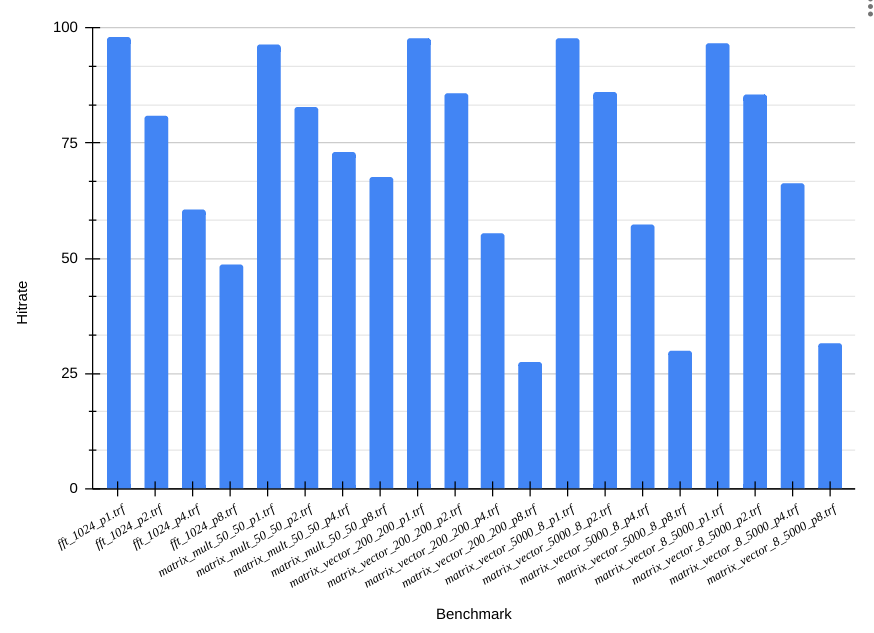
\includegraphics[scale=0.25]{Figures/Screenshot from 2024-03-06 05-33-36.png}
    \caption{Caption}
    \label{fig:enter-label}
\end{figure}
\\


The program also measures the average bus access times by recording the time intervals between the queueing of a cache request on the bus and the moment of its execution. The results show that overall, the access times do not vary much, except for some edge cases where the access time drops by around 15\% below the common average of 100 cycles. This seems to happen for the p2 benchmarks in the maxmul workload, specifically for grid sizes of 50x50 and 8x5000. However, the good news is that for larger numbers of cores, the average access time stays close to the 100-cycle mark.

\begin{figure}
    \centering
    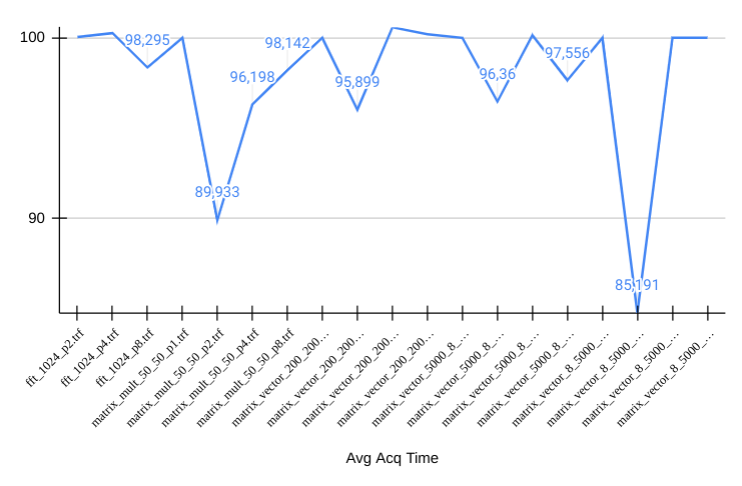
\includegraphics[scale=0.3]{Figures/Screenshot from 2024-03-06 05-53-53.png}
    \caption{Caption}
    \label{fig:enter-label}
\end{figure}

\\

\subsection{Conclusion}
The model seems to work reasonably well overall, but the bus is clearly a bottleneck in the system. To improve the performance, a potential enhancement could be to make the bus more asynchronous by allowing the caches to continue with computation while waiting for a response from a memory request. This could be achieved if there are subsequent reads to other cache lines that are ready to be used, effectively hiding the latency with computation. Furthermore, the model could assign priorities to the caches based on their level of activity, which might help in further optimizing the system's performance.




\newpage
\section{Assignment 3}

\subsection{Introduction}
For the part 3 of the assignment the goal is to build on top of the previous model done in part 2 and to implement the MOESI protocol instead of the simple V-I protocol. This requires the introduction of the new set of states and a more complex utilization of the bus with the addition of cache-to-cache communication.  


\subsection{MOESI Protocol}
The new cache states are VALID, EXCLUSIVE, SHARED, MODIFIED, OWNED. The state transition logic is based on the AMD illustration. The request system between slave and maters with the bus is largely unchanged from the previous model, and the bus receives the requests from cache and memory into two distinct queues, where the memory queue has priority as it returns the values back to the respective caches. The only change now is that the incoming tasks have an additional argument specifying whether it is a cache hit or not (request(addr, isWrite, id, busWB)). the second argument determines which kind of probe to launch in case there are matching lines in other caches, and is true it is used to invalided all the caches. The last parameter is used to perform write-back to memory actions without performing other checks. This action takes place only when a Modified or Owned line is evicted. The structure of the model is overall the same as for the assignment 2, but with additional signals and information data. The caches are now not only waiting for a memory signal (memory return), but also for a status update signal. More specifically, each action waits until one of the two signals is triggered. If the memory signal is triggered, it means there was no data found in other caches, thus leading, for example, to Exclusive state. If the state update signal is received, it means there are other copies in other caches.  
    

\subsection{Analysis}

For this part of the project we can finally compare 2 models with two different coherency policies, V-I and MOESI. In this section we will discuss speedups on matrix multiplication for both policies, total time differences, memory access differences, bus contention differences.

\subsubsection{Hitrates}
For our analysis we compared hitrates on 32kB cache sizes. The results show a very consistent behavior on the MOESI side, showing stable hitrates above 80\% for all of our tests. This might be due to the fact that overall MOESI is a more sophisticated model. Also, due to the deferrement of write-back in the MOESI protocol, this result seems reasonable. On the other hand, in \autoref{fig:ass2hit}, with the increase of cores we lose a substantial amount of hits. This might be due to the high amount of invalidations.
\begin{figure}[H]
    \centering
    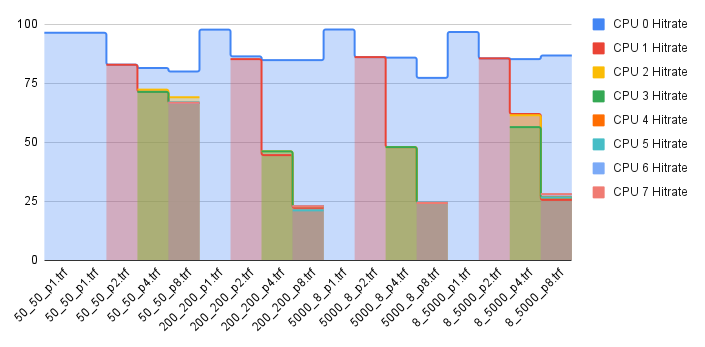
\includegraphics[scale=0.4]{Figures/ass2_hitrates.png}
    \caption{V-I hitrates}
    \label{fig:ass2hit}
\end{figure}
\begin{figure}
    \centering
    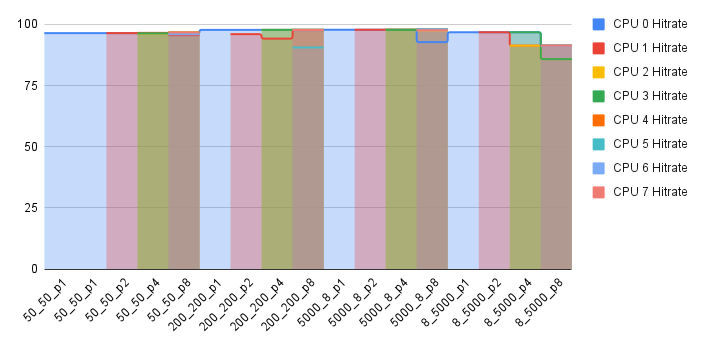
\includegraphics[scale=0.4]{Figures/ass3_hitrates.png}
    \caption{MOESI hitrates}
    \label{fig:ass3hit}
\end{figure}

\subsubsection{Speedup}
The speedup results are in line with the runitmes (\autoref{fig:runtime}) and the hitrates. As we can see in \autoref{fig:speedups}, the speedup is again more consistent on the MOESI model, even though not great. This is a great achievement when we compare it to the V-I perormance.
\begin{figure}[H]
    \centering
    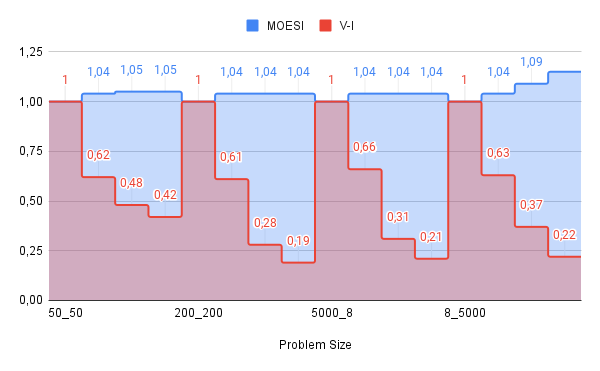
\includegraphics[scale=0.4]{Figures/speedups.png}
    \caption{Speedups}
    \label{fig:speedups}
\end{figure}

\subsubsection{Total run time}
The runtimes seem to also be much better performant in MOESI, with the greatest improvement observed on small problem sizes.
\begin{figure}[H]
    \centering
    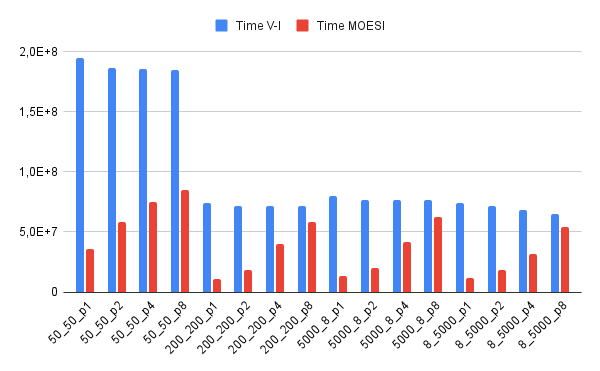
\includegraphics[scale=0.4]{Figures/time.png}
    \caption{Total runtimes}
    \label{fig:runtime}
\end{figure}


\subsubsection{Memory accesses}
An interesting factor to analyze is of course the amount of memory accesses by the new model compared to the old one. One of the main stregths of MOESI, by design, is the fact that caches can provide data to other caches when it is available, enabling to cut down on write backs. The expectation thus is to overall see a decrease in total time and amount of memory accesses. As shown in \autoref{fig:enter-label}, the blue is the dominant, which represent the number of reads in the V-I model. On the other hand the reads from MOESI are drastically decreased (represented by the yellow color). Finally, the writes do not present large differences (red and green).

\begin{figure}[H]
    \centering
    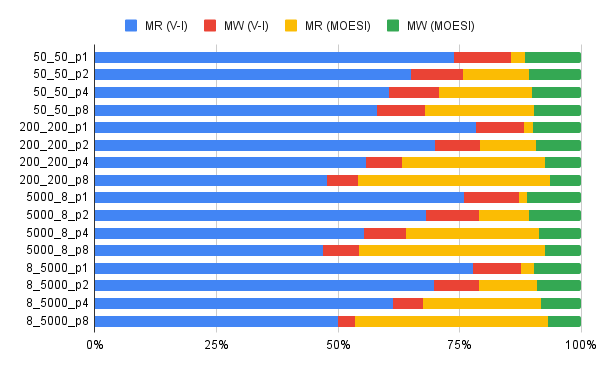
\includegraphics[scale=0.4]{Figures/memory accesses.png}
    \caption{Memory accesses}
    \label{fig:enter-label}
\end{figure}

\subsubsection{Average bus acquisition times}
With the implementation of a heavier state logic between the states and cache-to-cache communication, we expect to see the bus under greater stress compared to the V-I model. There should be a clear trade-off between decreased memory accesses and the fact that the bus becomes more of a bottleneck. In our implementation no arbitrer is implemented, thus the whole slaves-masters and masters-masters communication is handled by a single bus module. With the V-I model there could be at most n\_caches elements in the cache request queue on the bus, as the caches needed to wait for completion from memory. Now, we introduce a load of new elements to the queue that include cache-to-cache communications. Therefore, the average bus acquisition goes up. \autoref{fig:accessbus}, however, shows a small improvement on the MOESI side, which might probably be due to the implementation of the models or to the fact that even though there are more cache-to-cache transactions, there are also far less memory transactions.

\begin{figure}[H]
    \centering
    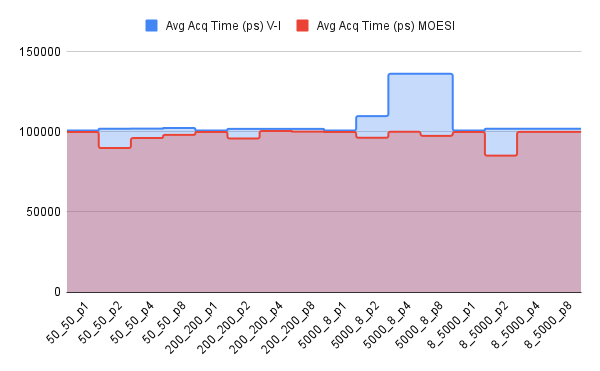
\includegraphics[scale=0.4]{Figures/avg_Access_bus.png}
    \caption{Average acquisition time}
    \label{fig:accessbus}
\end{figure}


\subsection{Conclusion and Possible improvements}
The MOESI protocol seems to be very reliable and efficient in reducing the latency of accessing memory and hides it with computation. The efficiency of the MOESI protocol can also be influenced by the replacement policies used in shared caches4. Exploring near-optimal replacement policies could lead to performance improvements. Additionally, to better exploit space locality in matrix multiplication applications, it could be beneficial to enhance the line transfers between caches with multiple adjacent lines to further decrease latency.